% This is samplepaper.tex, a sample chapter demonstrating the
% LLNCS macro package for Springer Computer Science proceedings;
% Version 2.21 of 2022/01/12
%
\documentclass[runningheads]{llncs}
%
\usepackage[T1]{fontenc}
% T1 fonts will be used to generate the final print and online PDFs,
% so please use T1 fonts in your manuscript whenever possible.
% Other font encondings may result in incorrect characters.
%
\usepackage{graphicx}
% Used for displaying a sample figure. If possible, figure files should
% be included in EPS format.
%
% If you use the hyperref package, please uncomment the following two lines
% to display URLs in blue roman font according to Springer's eBook style:
%\usepackage{color}
%\renewcommand\UrlFont{\color{blue}\rmfamily}
%\urlstyle{rm}
\usepackage[numbers]{natbib}
\usepackage{url}
\usepackage{amsmath}
\usepackage{subfig}
%
\begin{document}
%
\title{Hyperspectral Band Selection Using Metaheuristics for the Detection of \textit{Aspergillus flavus} in Figs with Machine Learning}
%
\titlerunning{Band Selection for \textit{Aspergillus flavus} Detection in Figs}
% If the paper title is too long for the running head, you can set
% an abbreviated paper title here
%
\author{Israel {Calder\'{o}n Aguilar}\inst{1}\orcidID{0009-0007-6396-2775} \and
        Juan {Villegas Cortez}\inst{1}\orcidID{0000-0001-8918-1044} \and
        Josefa {D\'{\i}az \'{A}lvarez}\inst{2}\orcidID{0000-0003-2105-3905} \and
        Rom\'{a}n Anselmo {Mora Gutiérrez}\inst{1}\orcidID{0000-0002-2112-7049} \and
        Francisco {Fernandez De Vega}\inst{2}\orcidID{0000-0002-1086-1483} \and
        Francisco {Ch\'{a}vez de la O}\inst{2}\orcidID{0000-0002-9565-743X} \and
        Ana {Mart\'{\i}nez Dorado}\inst{3} \and
        Roc\'{\i}o {Casquete Palencia}\inst{4}}
%
\authorrunning{Calder\'{o}n et al.}
% First names are abbreviated in the running head.
% If there are more than two authors, 'et al.' is used.
%
\institute{Systems Department, Universidad Autónoma Metropolitana, Unidad Azcapotzalco, Av. San Pablo 420, Col. Nueva El Rosario, Alc. Azcapotzalco, 02128 Mexico City, Mexico \\
\email{\{al2243804651,juanvc,mgra\}@azc.uam.mx}\and
Computer Architecture Department, University of Extremadura, C. Santa Teresa de Jornet, 38, 06800 Mérida, Spain \\
\email{\{mjdiaz, fcofdez, fchavez\}@unex.es}\and
Nutrición y Bromatología, Escuela de Ingenierías Agrarias, University of Extremadura, Avd. Adolfo Suárez s/n, 06007 Badajoz, Spain\\
\email{anamd@unex.es}\and
Instituto Universitario de Investigación en Recursos Agrarios (INURA), University of Extremadura, Avd. de la Investigación, 06006 Badajoz, Spain\\
\email{rociocp@unex.es}}
%
\maketitle % typeset the header of the contribution
%
\begin{abstract}
Hyperspectral Imaging offers a powerful non-invasive tool for precision agriculture; however, its inherent high dimensionality represents a computational challenge. This paper proposes a metaheuristic based intelligent framework to optimize band selection for the detection of severe \textit{Aspergillus flavus} infections in \textit{Ficus carica} (figs). The dataset utilized consists of 560 samples, strictly divided into 277 healthy controls and 283 samples inoculated with a high fungal concentration ($10^7$ CFU/mL). We comparatively evaluate Genetic Algorithms (GA) and Particle Swarm Optimization (PSO) to identify highly compact and discriminative spectral subsets. A core methodological contribution is the design of a concatenated feature vector combining mean reflectance and spatial standard deviation ($\mu + \sigma$), which successfully captures both spectral tendency and infection induced textural heterogeneity. To mitigate the computational overhead of the metaheuristic search, a two stage Support Vector Machine (SVM) evaluation strategy is implemented utilizing cross-validation, balancing rapid fitness estimation with rigorous hyperparameter fine tuning. Furthermore, a Shapley Additive Explanations (SHAP) analysis was conducted on the global optimum model to quantify feature weights and impact directionality. Experimental results demonstrate that GA outperforms PSO in navigating the search space, achieving a global maximum F1-Score of 0.836 on a held-out test set using an optimal subset of only 5 bands. The proposed framework drastically reduces data dimensionality while preserving classification accuracy, offering a scalable and explainable AI solution for automated food safety inspection.

\keywords{Hyperspectral Imaging \and Support Vector Machine \and Genetic Algorithm \and Particle Swarm Optimization \and Precision Agriculture.}
\end{abstract}
%
%
%
\section{Introduction}
Food safety and economic sustainability in agriculture face a constant threat due to contamination by pathogenic fungi. 
Among them, \textit{Aspergillus flavus} stands out for its dangerousness, as it is the main producer of aflatoxins, secondary metabolites classified as Group 1 human carcinogens, closely linked to the development of hepatocellular carcinoma \cite{cruz-carrasco_detection_2024}. 
The detection of this pathogen is critical, especially in high-value crops such as the fig (Ficus carica), where regions like Extremadura lead national production in Spain, which ranked as the world's seventh-largest producer in 2025 \cite{fao_fao_2025}. 
Traditionally, the identification of these mycotoxins has relied on analytical chemical methods (such as HPLC or ELISA), which, although precise, are destructive, expensive, and time-consuming, preventing the inspection of 100\% of the production \cite{chu_classifying_2020, park_hyperspectral_2015}. 
To overcome these limitations, the industry has turned towards non-invasive assessment methods. 
In this context, Hyperspectral Imaging (HSI) has emerged as a revolutionary tool. 
Unlike conventional computer vision, HSI technology captures detailed spectral information across hundreds of contiguous bands for each pixel of an image, allowing the detection of complex physicochemical changes and structural degradation in plant tissues that are often difficult to assess with the naked eye \cite{wang_review_2021, chu_classifying_2020}. 
However, the large amount of data generated by these images presents a significant challenge for their efficient processing.

The use of HSI for the detection of fungal diseases has been widely explored in the last decade. 
Previous research has demonstrated the efficacy of this technology in detecting aflatoxins and fungi in maize, peanuts, and other nuts \cite{park_hyperspectral_2015, cruz-carrasco_detection_2024}. 

With respect to figs, recent studies have applied deep learning techniques, such as Convolutional Neural Networks (CNN) and Fully Connected Neural Networks (FCNN), to detect the infection of \textit{Aspergillus flavus}~\cite{cruz-carrasco_detection_2024}. The results presented high accurary rates for classifying infected pixels. This research study set an important precedent by comparing deep neural network architectures on the same type of samples, and demonstrating the viability of a pixel-level analysis to accurately predict the presence of \textit{Aspergillus flavus}.

However, many of these approaches utilize the full spectrum, which requires expensive hardware and high computational power. 
Current literature suggests that spectral band selection is a crucial step for practical implementation \cite{sawant_survey_2020}. 
Statistical methods such as Principal Component Analysis (PCA) have traditionally been used to reduce data \cite{chu_classifying_2020}, but techniques based on evolutionary algorithms (such as GA and PSO) are gaining ground due to their ability to find global optimal solutions in complex search spaces \cite{sawant_survey_2020}.

The main objective of this research work is to optimize the detection of severe \textit{Aspergillus flavus} infections in fresh figs using an evolutionary approach. The feature engineering strategy involved the design of a concatenated statistical vector, evaluated through metaheuristic algorithms specifically Genetic Algorithms and Particle Swarm Optimization for intelligent spectral band selection. A Support Vector Machine (SVM) was applied to assess the fitness of the candidate subsets. Ultimately, this work aims to identify an optimal subset of spectral bands that significantly reduces the complexity of hyperspectral data without compromising detection capability, offering a scalable and explainable path for the agricultural industry.

\section{Materials and Methods}

The methodology employed in this work is structured into five sequential stages, as illustrated in Figure \ref{fig:1}. First, the acquisition of hyperspectral images of healthy and infected figs was carried out. The second stage consisted of image preprocessing, which included radiometric correction and region of interest (ROI) segmentation. In the third stage, feature extraction was performed to compute representative statistical metrics (mean and standard deviation) for each sample. Fourth, an optimization strategy based on metaheuristics was implemented and evaluated using a Support Vector Machine (SVM), with the objective of reducing dimensionality and selecting the optimal spectral bands for the detection of \textit{Aspergillus flavus}. Finally, in the fifth stage, a SHAP analysis was conducted on the global optimum model to interpret feature importance and directionality.

\subsection{Sample Preparation and Data Acquisition}

This research work utilized hyperspectral images previously acquired and analyzed using alternative classification strategies \cite{cruz-carrasco_detection_2024}. 

These images were generated using fresh figs (Ficus carica L.) of the \textit{Calabacita} variety, which were harvested at the "Finca La Orden-Valdesequera" belonging to the Scientific and Technological Research Center of Extremadura (CICYTEX), located in Guadajira, Badajoz, Spain. All the figs were harvested at the same time.

\subsubsection{Inoculation process}
The inoculation process was carried out under controlled conditions by agriculture engineers belonging to CICYTEX. The figs were arranged into four trays, each containing 36--40 fruits. One tray served as the healthy control group, while the figs in the remaining three trays underwent the inoculation process. 
As a first step, hyperspectral images for healthy controls were taken.

The inoculation involved submerging the lower portion of each fig in a solution containing a strain of \textit{Aspergillus flavus} for 4--5 seconds. This process ensures that the distribution of the fungus on the fig surface is comparable to natural contamination. Particularly, for this study, one strains from the collection of the CAMIALI group from the University of Extremadura, Spain (\textit{Aspergillus flavus} HG 144M) was used.

The protocol set during the inoculation process was designed to apply a solution containing three different concentrations of the fungi to the figs in the three specific trays. These concentrations were $10^3$ CFU/mL,  $10^5$ CFU/mL, and $10^7$ CFU/mL, identifying classes 1, 2 and 3, respectively. Quantification of \textit{Aspergillus flavus} was performed in CFU/mL to estimate the viable fungal load, considering only those units capable of proliferating on the cultivation medium. This approach is particularly relevant for assessing the potential for colonization.

Hyperspectral images were acquired every 24 hours for five consecutive days following inoculation. Between the acquisition sessions, samples were kept in a controlled-environment incubation chamber. The chamber was set at 25 °C with a relative humidity of $80-90\%$, providing environmental conditions optimized for fungal growth and development. Once data acquisition was finished the first subsequent downstream analysis started \cite{cruz-carrasco_detection_2024}.

Image acquisition was performed using a line-scan (pushbroom) hyperspectral camera, particularly the SPECIM model FX10.
The sensor of this camera captures information in the visible and near-infrared (VNIR) spectral range. 
This device features a spectral range from 400 nm to 1000 nm, and a spectral resolution of 448 bands with a spectral sampling interval of approximately 1.339 nm. 
Its spatial resolution is 1024 pixels in spatial width per scan line. For each acquired scene, 800 scan lines were captured, resulting in a final hyperspectral data cube dimension of 1024 x 800 x 448 (spatial width x scan lines x spectral bands) \cite{specim_specim_2020}.

In this work, not all images for all classes were used. The focus was on discriminating between healthy controls and samples inoculated with the high concentrations of the fungi, identified as class 3 ($10^7 CFU/mL$), which constituted the working dataset. This study addressed the binary classification between infected and non-infected samples. From now on, we will refer to these as classes 0 and 1, respectively.

As a summary, these samples are organized as follows:

\begin{itemize}
    \item Class 0: Healthy controls with non-inoculated figs, used as a reference for the healthy state of the fig.
    \item Class 1: Severe infection class. Figs inoculated with an \textit{Aspergillus flavus} concentration of $10^7 CFU/mL$, representing a high fungal load scenario.
\end{itemize}

\subsection{Data Preprocessing}
As previously mentioned, in the acquired images the figs were arranged on trays, each containing approximately 40 samples, and the evaluation needed to be conducted for each independent fig.  
To process the spectral information of each fruit individually, manual segmentation was performed using the open-source software LabelMe (v5.8.3) \cite{wada_wkentarolabelme_2021}. 
This process resulted in the processing of 18 hyperspectral scenes, yielding a total of 560 individual segmentation masks. 
Consequently, the final dataset consisted of 560 samples, distributed as 277 samples for the control class (Class 0) and 283 samples for the inoculated class (Class 1) with a spore concentration of $1\times10^7$ CFU/mL.

\begin{figure}[]
    \centering
    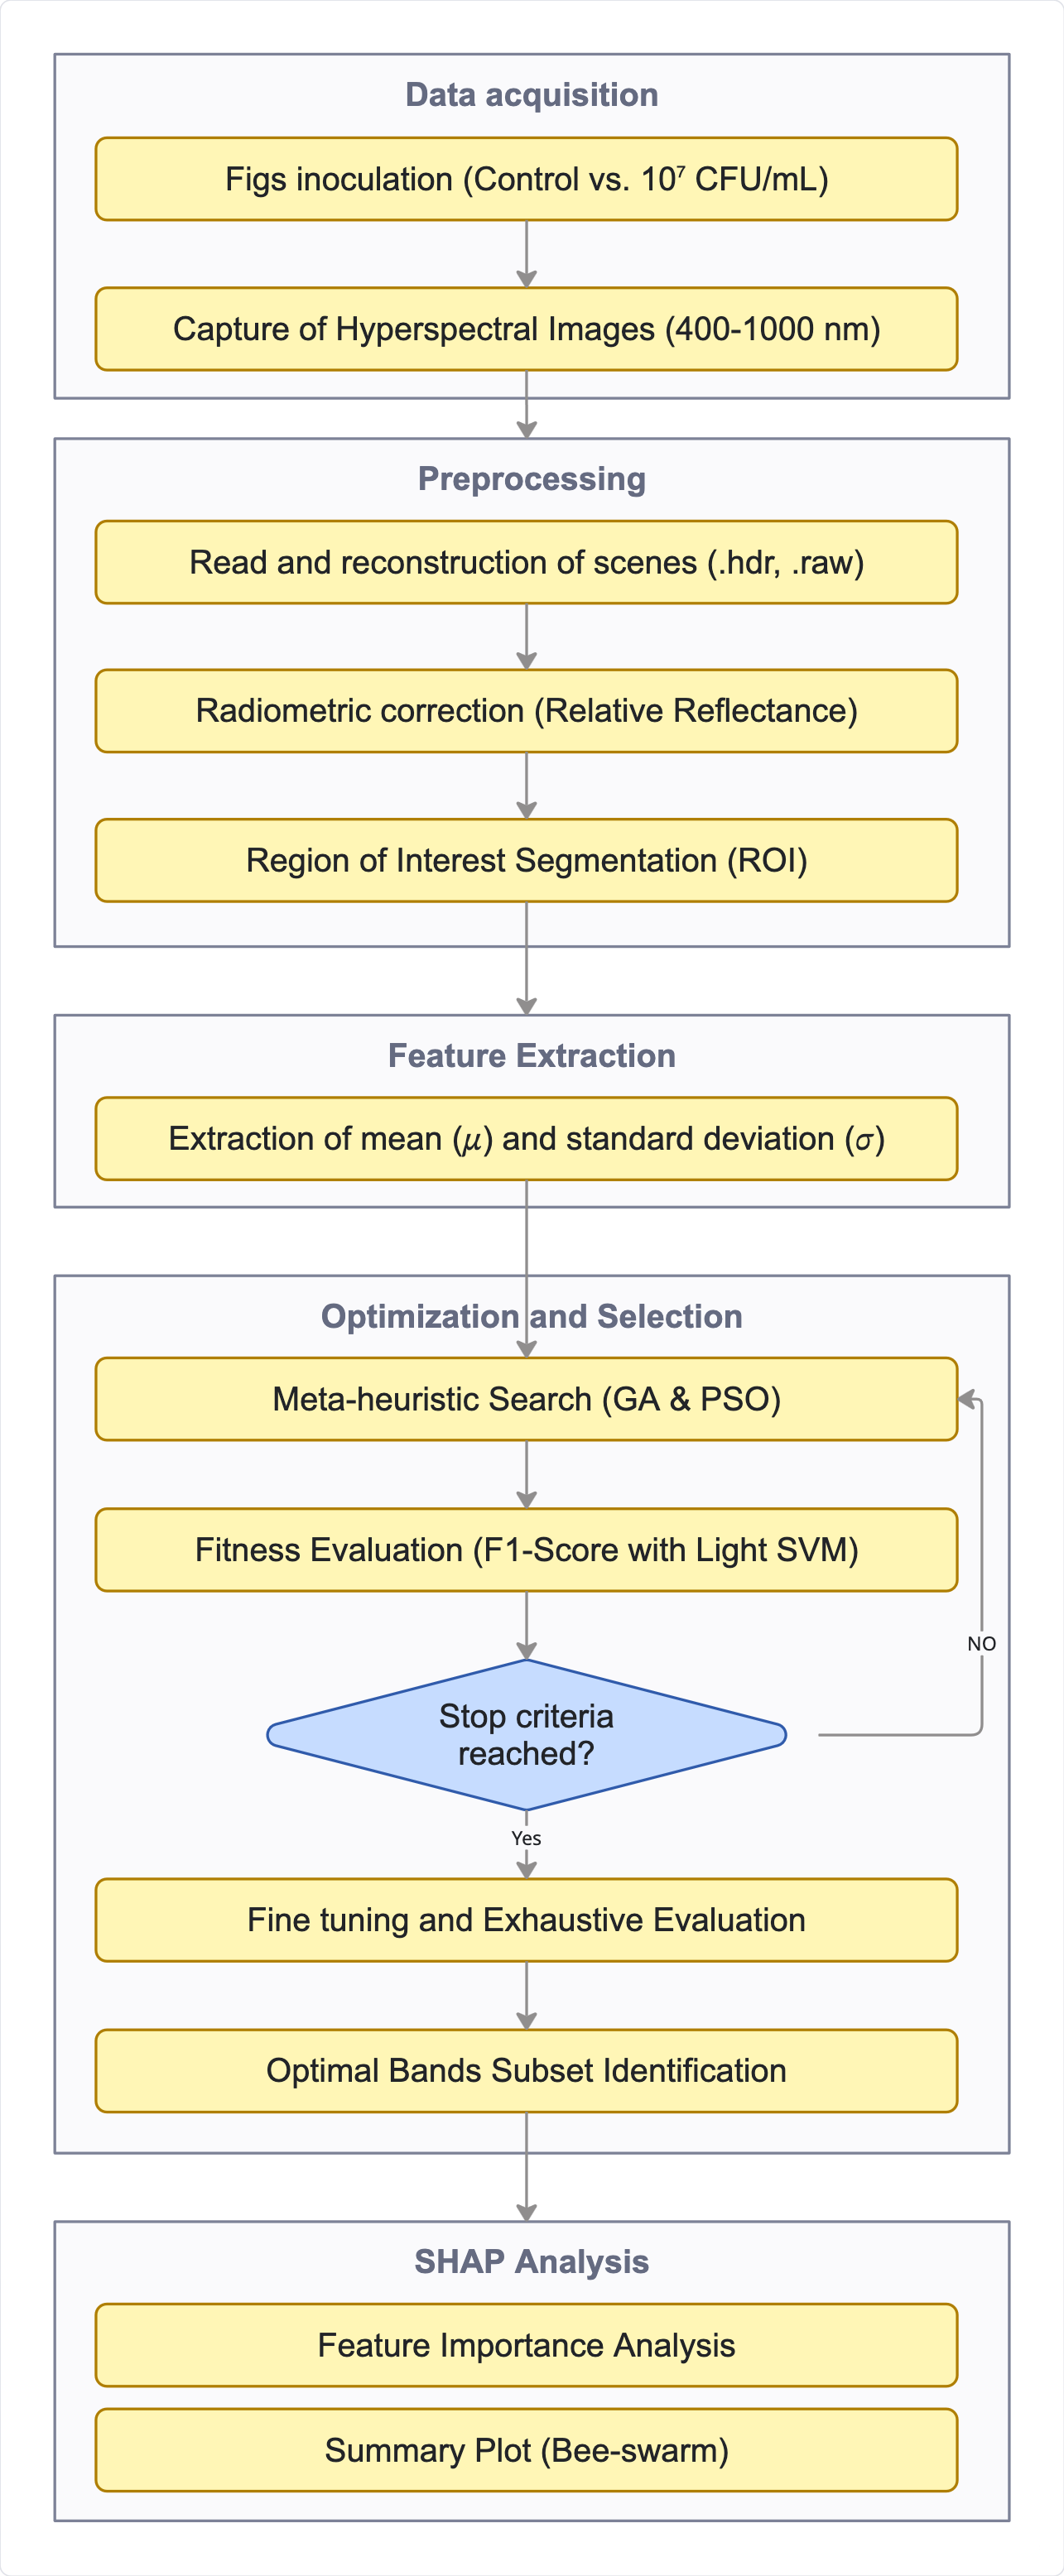
\includegraphics[width=0.7\textwidth]{images/framework_block_diagram.png}
    \caption{Flowchart of the proposed methodological framework, detailing the sequential pipeline from hyperspectral image acquisition to metaheuristic band selection and SHAP explainability analysis.\label{fig:1}}
\end{figure}


Data processing and feature extraction were conducted using the Spectral Python (SPy) library. 
First, the header (.hdr) and binary (.raw) files were read to reconstruct the hyperspectral data cubes. 
Raw intensity values were then converted into relative reflectance through radiometric calibration, using the white and dark references acquired with each scene, according to equation \cite{morales_laboratory_2022}:

\begin{equation}
    R=\dfrac{I_{raw}-I_{dark}}{I_{white}-I_{dark}}
\end{equation}

where $I_{raw}$ is the raw image, $I_{dark}$ is the dark reference, and $I_{white}$ is the white reference. 
Following calibration, spectral features were extracted from the previously segmented ROIs. 
For each sample (fig), the mean and standard deviation of the reflectance were calculated across all spectral bands. 
These values were stored in two distinct feature matrices; one representing the average spectral signatures and the other capturing spectral variability, which served as inputs for the subsequent band selection stages.

\subsection{Dimensionality Reduction and Band Selection}

Although hyperspectral imagery provides abundant information, it suffers from significant redundancy due to the high correlation between contiguous spectral bands \cite{sawant_survey_2020}. 
This characteristic leads to the called \textit{curse of dimensionality} or Hughes phenomenon, where classification accuracy tends to decrease as the number of spectral bands increases, given a limited number of training samples \cite{hughes_mean_1968}. 
This high redundancy is shown in the Figure \ref{fig:2} which is a correlation matrix of the spectral bands in the dataset generated of mean reflectance. 
The prominent structure formed in the diagonal of the matrix indicates groups of correlation coefficients near to 1.0. 
Furthermore, the high data volume significantly increases the computational burden required for processing. 
To address these challenges, band selection has proven to be an effective strategy for dimensionality reduction, eliminating redundancy while preserving the most discriminative spectral features \cite{sawant_survey_2020, nagasubramanian_hyperspectral_2018}. 
In this study, two metaheuristic approaches are employed for optimal band selection: GA and PSO. 

Comparing PSO and GA can provide valuable information to the problem at hand. PSO is more effective in exploiting the search space by quickly adjusting solutions near the optimum, but it can get trapped in local optima due to its tendency to rapidly focus on specific areas. In contrast, GA favors global exploration and diversity, avoiding premature convergence and being more robust in multimodal spaces. Comparing both algorithms can help to identify whether the problem will require more exploration, where GA excels, or more exploitation, where PSO is more efficient. Not only will this improve the efficiency and robustness in the search for global optima, but it also can provide valuable insights to guide the next research steps.

\begin{figure}
\centering
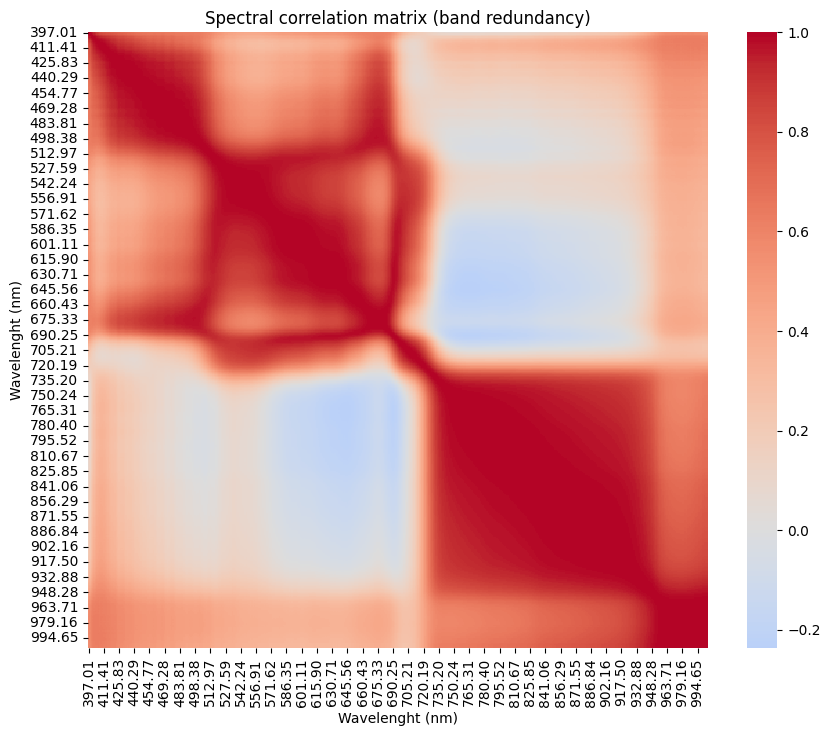
\includegraphics[width=0.8\textwidth]{images/spectral_colrrelation_matrix.png}
\caption{Figs mean values correlation matrix.}
\label{fig:2}
\end{figure}

\subsubsection{Feature Construction and Optimization Problem}

To thoroughly capture the impact of fungal infection on both spectral response and surface texture, a concatenated feature vector was constructed combining the mean ($\mu$) and standard deviation ($\sigma$) of the reflectance values across all the pixels within the ROI for each spectral band. 
The mean reflectance characterizes the central tendency of the spectral signature \cite{nagasubramanian_hyperspectral_2018}, while the standard deviation quantifies the spatial variability of the sample surface \cite{hossain_color_2019}. 
Formally, for a hyperspectral image with $n$ bands, the complete pool of available features for the $i$-th sample is defined as $Xi=[\mu_{i,1},\ldots \mu_{i,n},\sigma_{i,1},\ldots,\sigma_{i,n}]$. 
However, to maintain spectral consistency, the dimensionality reduction process was formulated as a band selection problem rather than an individual feature selection task. 
This means that selecting the $j$-th spectral band implies the simultaneous inclusion of both its corresponding mean ($\mu_j$) and standard deviation ($\sigma_j$) into the classifier input vector.

Therefore, the optimization search space consists of $n$ binary variables (where $n$ is the number of bands), but the dimensionality of the resulting feature vector sent to the classifier is $ 2\times{k} $, where $k$ is the number of selected bands. 
The objective is to find the binary vector $B=\{b_1,\ldots,b_n\}$ that maximizes the F1-Score \eqref{eq:f1_score}.

\begin{equation} \label{eq:f1_score}
    F1=2\times{\frac{Precision \times{Recall}}{Precision + Recall}}
\end{equation}


The F1-Score was selected as the fitness function due to its ability to balance precision and recall. 
It is critical to penalize false negatives (infected figs misclassified as healthy), as these represent a significant health risk. 
Furthermore, the F1-Score provides a robust performance metric that effectively mitigates the bias potentially introduced by the slight class imbalance in the dataset.
While the F1-Score explicitly drove the evolutionary search, a comprehensive evaluation including Accuracy, Precision, and Recall is provided in the final model assessment to ensure overall classification reliability.

\subsubsection{Genetic Algorithm}
The Genetic Algorithm is a metaheuristic optimization technique bio-inspired by natural evolution and genetic recombination. 
It encodes candidate solutions (individuals) as vectors and iteratively applies evolutionary operators such as selection, crossover, and mutation, often supplemented by elitism strategies \cite{eiben_introduction_2015, deb_multi-objective_2001}. 
This implementation used a 448-bit binary string to encode the band subset, where a value of "1" indicates selection, and a "0" value denotes exclusion.
The algorithm evolves the population over successive generations to optimize the target fitness function. 
The specific parameter settings used in this study are detailed in Table \ref{tab1}.

\begin{table}
    \caption{Genetic Algorithm parameters.\label{tab1}}
    \centering
    \begin{tabular}{ll}
        \hline
        {\bfseries Parameter} & {\bfseries Value}\\
        \hline
        Independent runs & 30 \\
        Generations & 350\\
        Population & 250\\
        Selection & Tournament ($k=5$) \\
        Crossover & Single Point \\
        Crossover Probability & 1.0\\
        Mutation rate & 25\%\\
        Elitism & 2 best individuals\\
        \hline
    \end{tabular}
\end{table}

\subsubsection{Particle Swarm Optimization Algorithm}
Particle Swarm Optimization is a stochastic metaheuristic inspired by the collective social behavior of bird flocks and fish schools. 
Unlike traditional evolutionary algorithms that rely on recombination or crossover operators, PSO models the population members as particles traversing an n-dimensional search space. By analogy, a swarm is similar to a population and a particle is similar to an individual.   
Each particle is characterized by its current position (representing a candidate solution for the band selection) and a velocity vector that governs its trajectory. 
The movement of a particle is determined by updating its velocity based on a weighted sum of three distinct components (inertia, cognitive and social) \cite{eiben_introduction_2015}.

To enhance convergence efficiency and mitigate premature convergence to local optima, Time-Varying Acceleration Coefficients (TVAC) were implemented. The inertia component was set at a fixed value.
The cognitive coefficient ($C1$) was linearly decremented to encourage exploration during the early stages, while the social coefficient ($C2$) was linearly incremented to promote global exploitation towards the end of the search process. 
The dynamic adjustment of these parameters follows standard literature recommendations for high-dimensional optimization \cite{ratnaweera_self-organizing_2004}. 

\begin{equation}
    c_1(t)=(c_{1,f}-c_{1,i}) \frac{t}{T_{max}}+C_{1,i}
\end{equation}
\begin{equation}
    c_2(t)=(c_{2,f}-c_{2,i}) \frac{t}{T_{max}}+C_{2,i}
\end{equation}

Where:
\begin{itemize}
    \item $t$: Current iteration.
    \item $T_{max}$: Maximum number of iterations.
    \item $C_{1,i}$,$C_{2,i}$: Coefficient initial values.
    \item $C_{1,f}$,$C_{2,f}$: Coefficient final values.
\end{itemize}
The specific parameter settings used in this study are detailed in Table \ref{tab2}.

\begin{table}
    \centering
    % \small
    % \setlength{\tabcolsep}{3pt}
    \caption{PSO parameters.\label{tab2}}
    \begin{tabular}{ll}
        \hline
        {\bfseries Parameter} & {\bfseries Value}\\
        \hline
        Independent runs & 30 \\
        Iterations & 650\\
        Particles & 200\\
        C1 & 0.4 to 2.5\\
        C2 & 2.5 to 0.4\\
        Inertia & 0.7\\
        Mutation rate & 0.2\\
        \hline
    \end{tabular}           
\end{table}

\subsection{Classification Model}
A SVM was implemented for the supervised classification task, selected for its proven robustness in high-dimensional spaces and effectiveness with limited datasets \cite{nagasubramanian_hyperspectral_2018, musci_ice_2020}. 
Given the non-linear nature of the spectral boundaries between healthy and infected samples, the Radial Basis Function (RBF) kernel was employed.

\subsubsection{Computational Strategy}
To mitigate the high computational overhead inherent to the iterative metaheuristic process (GA and PSO), a two stage evaluation strategy was implemented:
\begin{enumerate}
    \item Fast evaluator: A lightweight SVM configuration used as the wrapper within the fitness function. Its primary goal is to rapidly estimate how well perform the selected bands to guide the search algorithm, prioritizing the execution speed over hyperparameter tuning.
    \item Exhaustive evaluator: A rigorous final model, fine tuned via exhaustive hyperparameter search.
\end{enumerate}

\subsubsection{Validation Strategy and Data Splitting}
To ensure robust evaluation and prevent information leakage during the metaheuristic search, a strict data splitting protocol was enforced. For each of the 30 independent algorithmic runs, the dataset of 560 samples was partitioned into an 80\% training set and a 20\% held out test set using stratified random sampling.It is critical to note that the metaheuristic optimization loop (including the 3-fold cross-validation used by the fast SVM evaluator to calculate fitness) operated exclusively on the 80\% training set. The 20\% test set remained completely unseen during the evolutionary search and hyperparameter tuning phases. It was utilized strictly for the final evaluation of the global optimum model (the exhaustive evaluator), ensuring that the reported performance metrics reflect the model's true generalization capability on novel data.Regarding potential sample non-independence, it is acknowledged that the samples were extracted from four physical trays imaged independently. While batch effects (e.g., micro-environmental or lighting variations per tray) are a common challenge in hyperspectral imaging, a tray-level cross-validation strategy (leave-one-tray-out) could not be implemented for this specific binary task. Because the healthy controls and the severe infection class ($10^7$ CFU/mL) were inherently physically isolated on separate trays during the inoculation protocol, leaving out a tray would eliminate an entire class from either the training or testing phase. Therefore, sample-level stratified splitting was employed as the most rigorous available alternative, though mitigating potential batch effects via multi-tray sampling per class remains a priority for future data collection campaigns.

Before training, data normalization, using StandardScaler, was applied to ensure that both feature types (mean reflectance and standard deviation) contribute equally to the distance calculation. 
Finally, to ensure an unbiased evaluation, the winning model is evaluated on a test set that remained unseen during the optimization phase. 
The configuration parameters for both implementations are detailed in Table \ref{tab3}.

\begin{table}
    \centering
    \caption{SVM Parameters.\label{tab3}}
    \begin{tabular}{l|l|l}
        \hline
        Parameter & Fast Evaluator & Exhaustive Evaluator \\
        \hline
        Kernel & RBF & RBF \\
        Regularization ($C$) & Fixed 1.0 & Grid search 0.1 to 1000 \\
        Gamma ($\gamma$) & Fixed scale & Grid search 0.001 to 1 \\
        Validation Method & k-fold CV ($k=3$) & k-fold CV ($k=5$) \\
        \hline
    \end{tabular}
\end{table}

\section{Results}
\subsection{Spectral Characterization of Samples}
Figure \ref{fig:3}a displays the average spectral signatures relative to the healthy and infected fig samples across the full acquired spectral range (400--1000 nm). 
The shaded regions represent the standard deviation, illustrating the spectral variability within each class. 
As observed, the spectral patterns of both classes are visually similar, particularly in the visible region (400--700 nm). 
However, slight differences in reflectance intensity become more apparent in the Near Infrared (NIR) region (700--1000 nm), likely due to the structural degradation of the fig tissue caused by fungal colonization.
This high spectral overlap confirms the complexity of the classification task. 
Figure \ref{fig:3}b presents the standard deviation per wavelength. Visually, it is observed that infected samples exhibit greater variability compared to healthy controls, particularly across the visible and red-edge regions. To quantitatively validate this observation and verify that the curves represent distinct textural profiles, a Wilcoxon signed-rank test was applied to evaluate the differences between the spectral signatures. The test confirmed a highly statistically significant difference between the healthy and infected standard deviation curves ($p < 0.001$). This quantitative evidence firmly corroborates the premise that \textit{Aspergillus flavus} infection measurably alters the structural heterogeneity of the fig skin, providing a mathematically sound basis for including spatial standard deviation in the feature engineering pipeline.

\begin{figure}
\centering
\subfloat[]{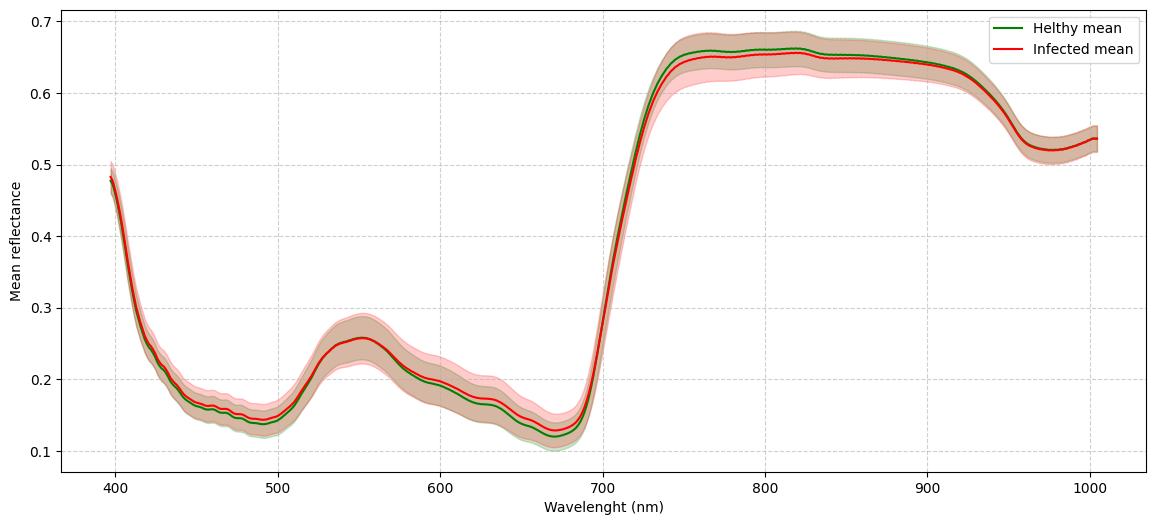
\includegraphics[width=0.8\textwidth]{images/spectral_signature_mean_reflectance.png}}\\
\subfloat[]{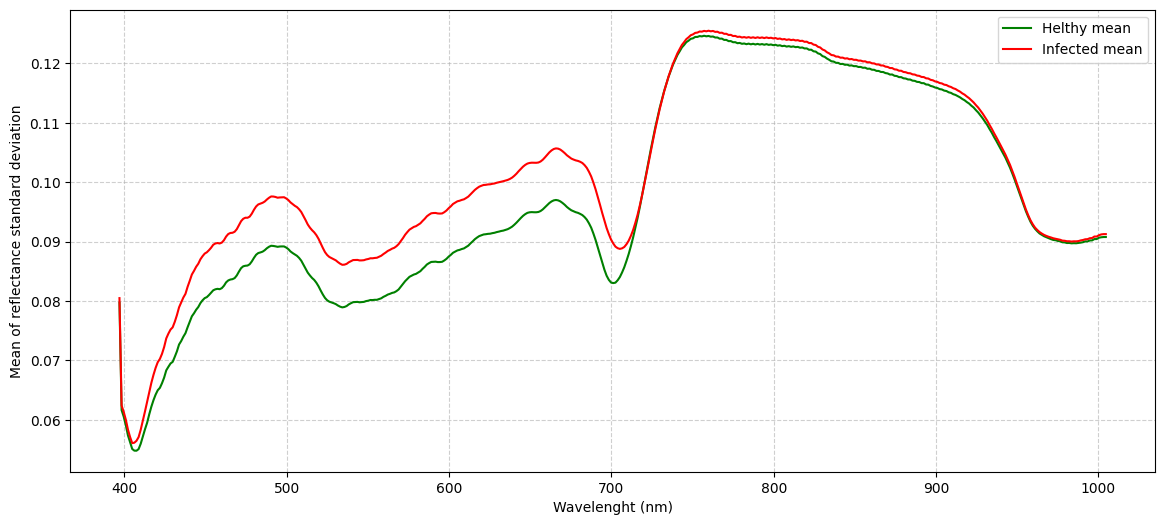
\includegraphics[width=0.8\textwidth]{images/spectral_signature_mean_standard_deviation.png}}
\caption{Spectral characterization of the fig samples. (\textbf{a}) Average reflectance signatures. (\textbf{b}) Standard deviation signatures.\label{fig:3}}
\end{figure}

\subsection{Impact of Feature Construction}
To validate the contribution of the standard deviation to the fungal classification, the band selection process was executed under two distinct feature configurations. 
Initially, the optimization was performed using only the mean reflectance per band, followed by a second scenario utilizing the combined mean and standard deviation vector. 
The optimization was conducted for target subset sizes of $k\in\{3,5,6\}$ over 30 independent runs. 
Table \ref{tab-metaheuristic-comparison} compares the average F1-Score obtained by the GA and PSO across both configurations.

In addition to the previous performance metrics, the evolutionary behavior of the optimization process was analyzed.
Figure \ref{fig:4} illustrates the average convergence history over 30 independent runs for both feature configurations. 
The solid lines represent the mean best fitness value at each generation, while the shaded regions indicate the standard deviation across runs.

\begin{table}
\centering
\caption{Improvement (\%) represents the relative percentage increase in the average F1-Score when utilizing the combined ($\mu + \sigma$) feature vector compared to the baseline mean-only ($\mu$) configuration.\label{tab-metaheuristic-comparison}}
\begin{tabular}{c|c|c|c|c|c|c}
\hline
Subset Size & Algorithm & Avg. F1-Score & Avg. F1-Score & Improvement & Best F1-Score & Best F1-Score\\
($k$) & & ($\mu$) & ($\mu + \sigma$) & ($\%$) & ($\mu$) &  ($\mu + \sigma$)\\
\hline
3 Bands & GA & 0.663 & 0.755 & +13.9\% & 0.704 & 0.817\\
 & PSO & 0.649 & 0.756 & +16.5\% & 0.679 & 0.807\\
\hline
5 Bands & GA & 0.698 & 0.770 & +10.3\% & 0.754 & 0.836\\
 & PSO & 0.697 & 0.699 & +0.3\% & 0.736 & 0.762\\
\hline
6 Bands & GA & 0.721 & 0.773 & +7.2\% & 0.817 & 0.820\\
 & PSO & 0.748 & 0.765 & +2.3\% & 0.832 & 0.821\\
\hline
\end{tabular}
\end{table}

\begin{figure}[!ht]
    \centering
    \subfloat[]{
\includegraphics[width=0.5\textwidth]{images/mean_convergence_3b.png}}
    \subfloat[]{
\includegraphics[width=0.5\textwidth]{images/mean_convergence_5b.png}} \\
    \subfloat[]{
\includegraphics[width=0.5\textwidth]{images/mean_convergence_6b.png}}
    \caption{Genetic Algorithm convergence profiles: (\textbf{a}) 3 bands; (\textbf{b}) 5 bands; and (\textbf{c}) 6 bands optimization scenarios.\label{fig:4}}
\end{figure}

It can be observed that the Combined Features ($\mu+\sigma$) strategy (represented by the blue line) not only starts with a higher initial fitness but also maintains a superior trajectory throughout the generations compared to the Mean Reflectance Only approach.  
This convergence gap visually confirms that the additional textural information provides a more robust search space, allowing the proposed algorithm to find higher quality solutions more efficiently.

To establish a classical dimensionality reduction baseline and validate the necessity of the metaheuristic search, Principal Component Analysis (PCA) was applied to the complete concatenated feature space (448 means + 448 standard deviations). The dataset was reduced to 5 principal components to exactly mirror the optimal subset size ($k=5$) selected by the GA. These components were subsequently evaluated using the exact same exhaustive SVM configuration and cross-validation strategy. The PCA-SVM baseline achieved an F1-Score of 0.648, which is substantially lower than the maximum 0.836 achieved by the proposed GA framework. Furthermore, an analysis of the PCA loadings revealed that the principal components were primarily driven by mean reflectance variance in the 450 nm and 805 nm regions, missing the critical spatial standard deviation markers at the red edge (707.93 nm and 763.94 nm) identified by the evolutionary search. This quantitative performance gap of over $28\%$ confirms that standard variance-based reduction is insufficient for this classification task, and proves that the metaheuristic algorithm successfully navigated the high-dimensional space to extract a highly discriminative subset of features.

\subsection{Comparative Analysis of Metaheuristic Algorithms}
After the validation of the feature construction, the study focused on comparing the optimization capabilities of the GA versus PSO. 
To ensure statistical robustness, both algorithms were executed 30 times for each target subset size ($k\in\{3,5,6\}$) using the combined feature vector.

The figure \ref{fig:5}a presents the boxplots summarizing the distribution of the F1-Scores obtained. 
The analysis reveals that the GA has a marginal difference with PSO in the context of hyperspectral band selection. 
Specifically, GA exhibited a higher median F1-Score when $k=\{5, 6\}$ subset sizes, particularly in the most scenario (k=6), where it achieved a median value of 0.773. 
However, PSO had a slight advantage in the 3 bands scenario. 
Furthermore, the interquartile ranges for GA were consistently narrower compared to PSO, indicating superior algorithmic stability and reproducibility.

%\begin{figure}[!ht]
%\centering
%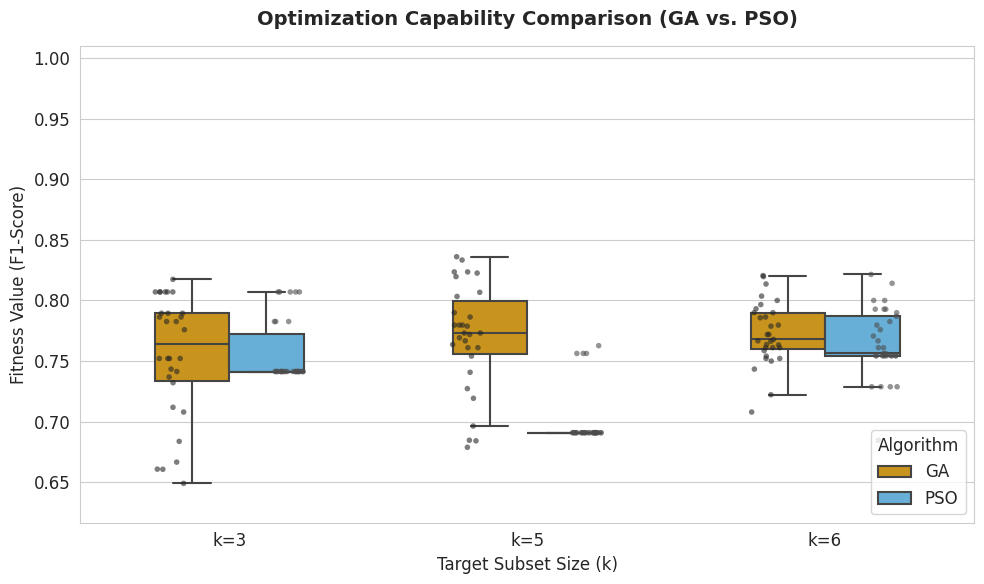
\includegraphics[width=0.8\textwidth]{images/boxplot_comparison_mean_std.png}
%\caption{Boxplot comparison GA vs. PSO with ($\mu+\sigma$) features.}
%\label{fig:5}
%\end{figure}
Notably, the absolute maximum F1-Score of the entire study (0.836) was achieved by the GA using the 5 band subset with the ($\mu+\sigma$) configuration. 
The specific wavelength found by this best individual were: 397.01, 398.32, 404.86, 707.93 and 763.94 nm. 
However, it is noteworthy that the configuration using only the mean ($\mu$) with 6 bands yielded a nearly identical score of 0.832. 
This suggests that the inclusion of the standard deviation stabilizes the search process and improves classification performance when the feature subset is small (e.g., 3 bands); however, this advantage diminishes as more bands are added. 
Figure \ref{fig:5}b illustrates this phenomenon, showing how the variance in the solution space increases for the 6-band configuration that relies solely on the mean.

To mathematically substantiate the performance differences observed between the algorithmic configurations, a non-parametric statistical analysis was conducted. Specifically, a Wilcoxon rank-sum test was applied across the 30 independent runs for each target subset size, utilizing a significance level of $\alpha = 0.05$. The statistical test confirmed that the Genetic Algorithm significantly outperformed Particle Swarm Optimization in the optimal 5-band scenario ($p < 0.001$). Furthermore, an identical test was executed to compare the feature construction strategies. The results statistically validated that the concatenated feature vector ($\mu + \sigma$) yields significantly higher F1-Scores than the baseline mean-only ($\mu$) configuration ($p < 0.001$), definitively proving that the inclusion of spatial standard deviation provides a crucial discriminative advantage for the metaheuristic search.

\begin{figure}[!ht]
    \centering
    \subfloat[]{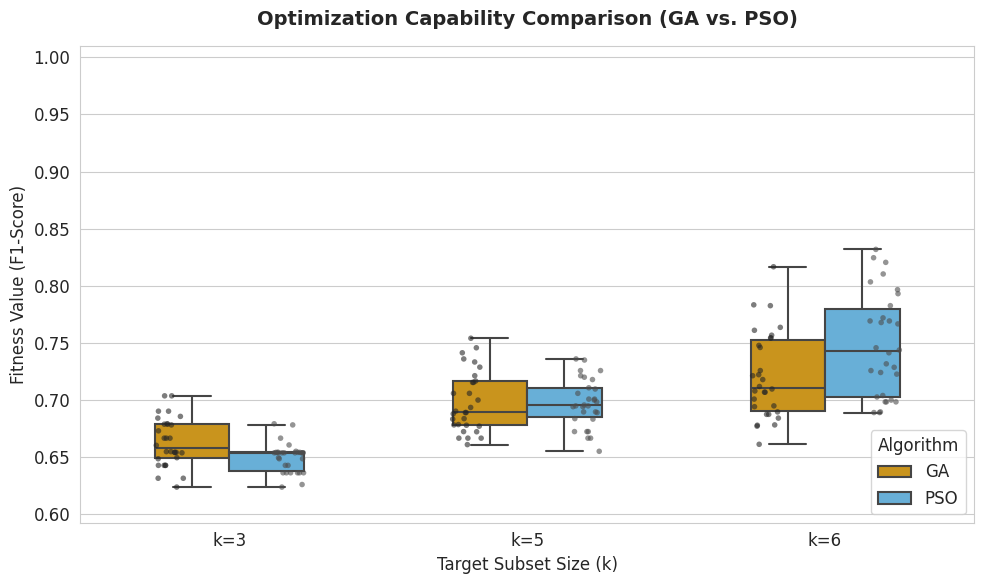
\includegraphics[width=0.5\textwidth]{images/boxplot_comparison_mean.png}}
    \subfloat[]{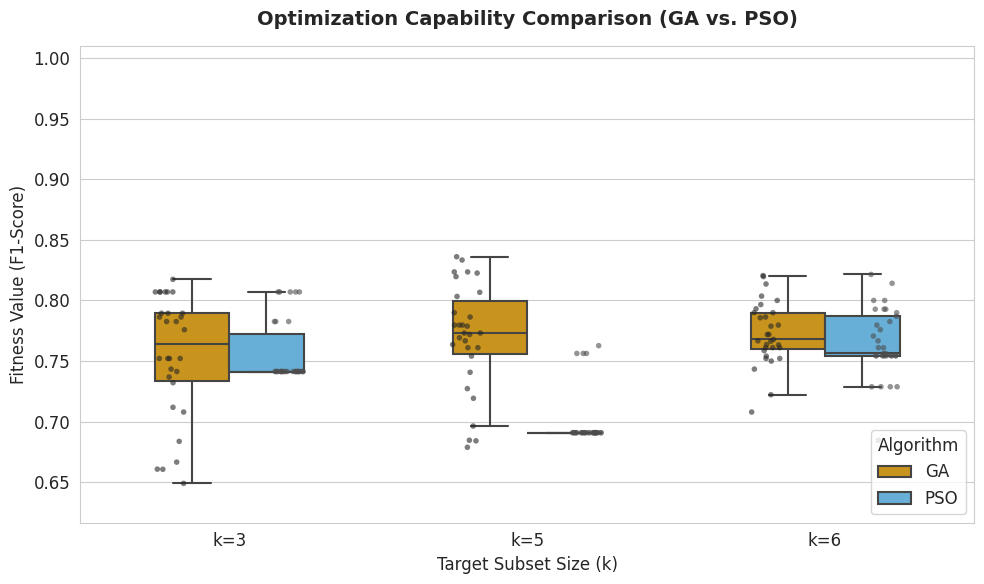
\includegraphics[width=0.5\textwidth]{images/boxplot_comparison_mean_std.png}}
    \caption{(\textbf{a}) Boxplot comparison GA vs. PSO only with ($\mu$) feature. (\textbf{b}) Boxplot comparison GA vs. PSO with ($\mu+\sigma$) features.}
    \label{fig:5}
\end{figure}

To provide a comprehensive evaluation of the optimal 5 bands GA model, Table \ref{tab6} details the Precision, Recall, F1-Score, and overall Accuracy achieved on the held out test set. While the model achieves a strong overall accuracy of 82\%, the most significant metric for food safety application is the 0.89 Recall for Class 1. This demonstrates that the metaheuristic subset is highly sensitive to the presence of \textit{Aspergillus flavus}, successfully identifying 89\% of all severe infections. This confirms that selecting the F1-Score as the fitness function successfully guided the algorithm to minimize critical false negatives (infected samples misclassified as healthy) while maintaining reliable overall precision.   

\begin{table}
    \centering
    \caption{Comprehensive performance metrics for the optimal GA subset (5 bands, $\mu + \sigma$) on the held out test set.\label{tab6}}
    \begin{tabular}{l|l|l|l}
        \hline
        Metric & Class 0 (Healthy) & Class 1 (Infected) & Macro Average \\
        \hline
        Precision & 0.87 & 0.78 & 0.83 \\
        Recall & 0.75 & 0.89 & 0.82 \\
        F1-Score & 0.80 & 0.84 & 0.82 \\
        Accuracy & - & - & 0.82 \\
        \hline
    \end{tabular}
\end{table}

\subsection{Comparative Analysis with Deep Learning Baselines}
To contextualize the performance of the proposed metaheuristic framework, it is imperative to compare it against prior deep learning approaches applied to the same dataset. Cruz-Carrasco et al. \cite{cruz-carrasco_detection_2024} previously analyzed these samples using pixel level deep learning models, specifically a Fully Connected Neural Network (FCNN) and a Convolutional Neural Network (CNN). Their work formulated a four class classification problem (healthy controls versus three varying infection concentrations) utilizing the entire 448-band spectral spectrum. Their best performing FCNN model achieved an overall F1-measure of 0.8325, with a specific F1-score of 0.87 when classifying the most severe infection class ($10^7$ CFU/mL).

\section{Model Interpretability and Physical Analysis (XAI)}
In feature spaces of high dimensionality such as those covered in this work, Suport Vector Machines equipped with non linear kernels operate as if they where black boxes, they obscure the underlying logic for the decision making. 
To ensure that the proposed methodology relies on true biological markers rather than circumstantial data, a Shapley Additive Explanations (SHAP) analysis was conducted on the global optimum model. 

To quantify the weight of each feature in the classifier decision, a SHAP feature importance analysis was generated by calculating the mean absolute SHAP values.
The quantitative ranking revealed that the mean reflectance at 707.93 nm and its corresponding spatial standard deviation are the most predominant features driving the classifier.
They are followed closely by the spatial standard deviation at 763.94 nm. Remarkably, two out of the top three most impactful features in the study belong to the standard deviation vector. 
This provides proof that capturing spatial textural heterogeneity is as important as measuring the mean reflectance. 

Furthermore, a SHAP summary plot (Beeswarm) was generated. This graphic reveals strong directional impacts that are highly consistent with plant pathology. 
The physical interpretation of the optimal 5 band subset demonstrates that the GA converged exclusively on two distinct physiological clusters: 

\begin{itemize}
    \item Red edge (707.93 and 763.94 nm): Holding the highest quantitative weight in the model, the standard deviation features in this cluster exhibit a clear unidirectional contribution. High spatial variability (represented by high-value red dots) heavily impacts the SHAP value in favor of the infected class. This indicates that the SVM leverages textural roughness caused by surface mycelium proliferation and cell wall degradation at the red edge as its primary diagnostic mechanism.
    \item Visible/Near UV (397.01, 398.32, and 404.86 nm): Forming a second cluster, these bands show that low mean reflectance values (blue dots) strongly push the model's prediction toward the infected class. This indicates that the infection by \textit{Aspergillus flavus} induces tissue darkening and necrosis, thereby increasing light absorption and lowering surface reflectance.
\end{itemize}

An interesting observation is that this optimal subset achieved the maximum classification F1 Score of 0.836 without selecting any bands in the water absorption region (950-1000 nm). 
This finding proves that early pigment alterations and textural stress markers are sufficiently discriminative for automated inspection, providing a highly explainable and computationally efficient AI solution.
\begin{figure}[!ht]
    \centering
    \subfloat[]{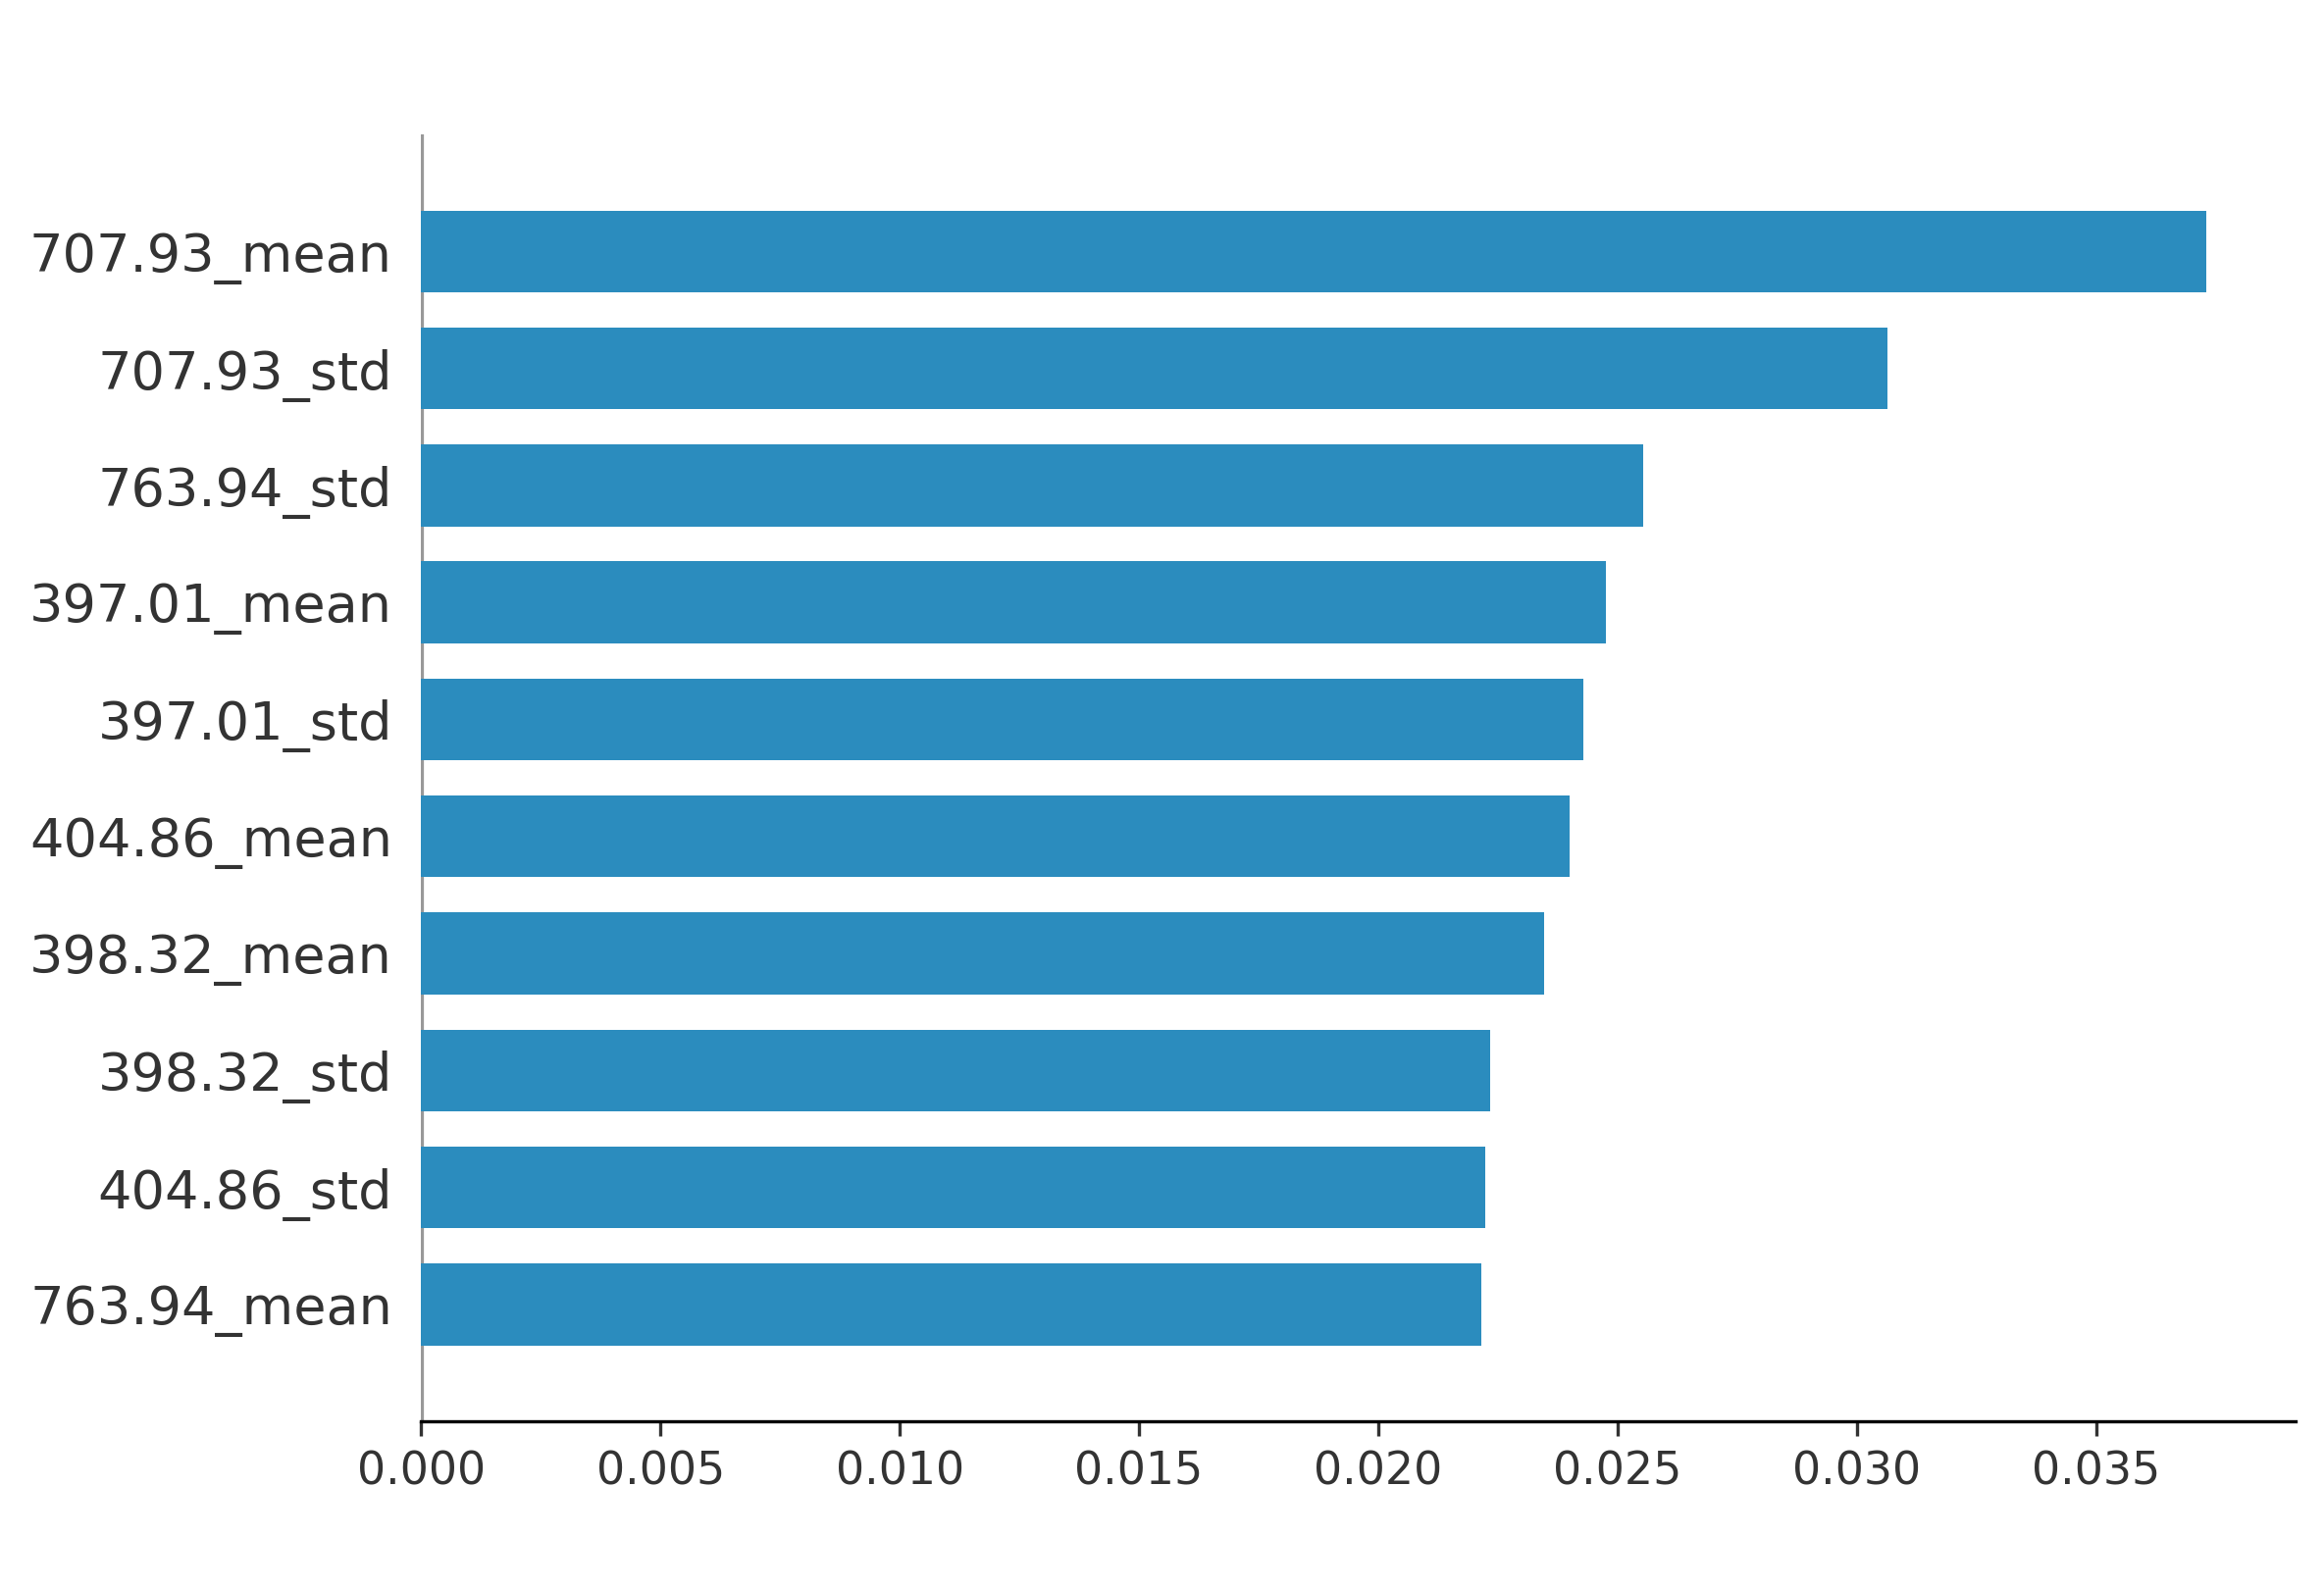
\includegraphics[width=0.5\textwidth]{images/shap_bar_plot_ga_5_bands.png}}
    \hfill
    \subfloat[]{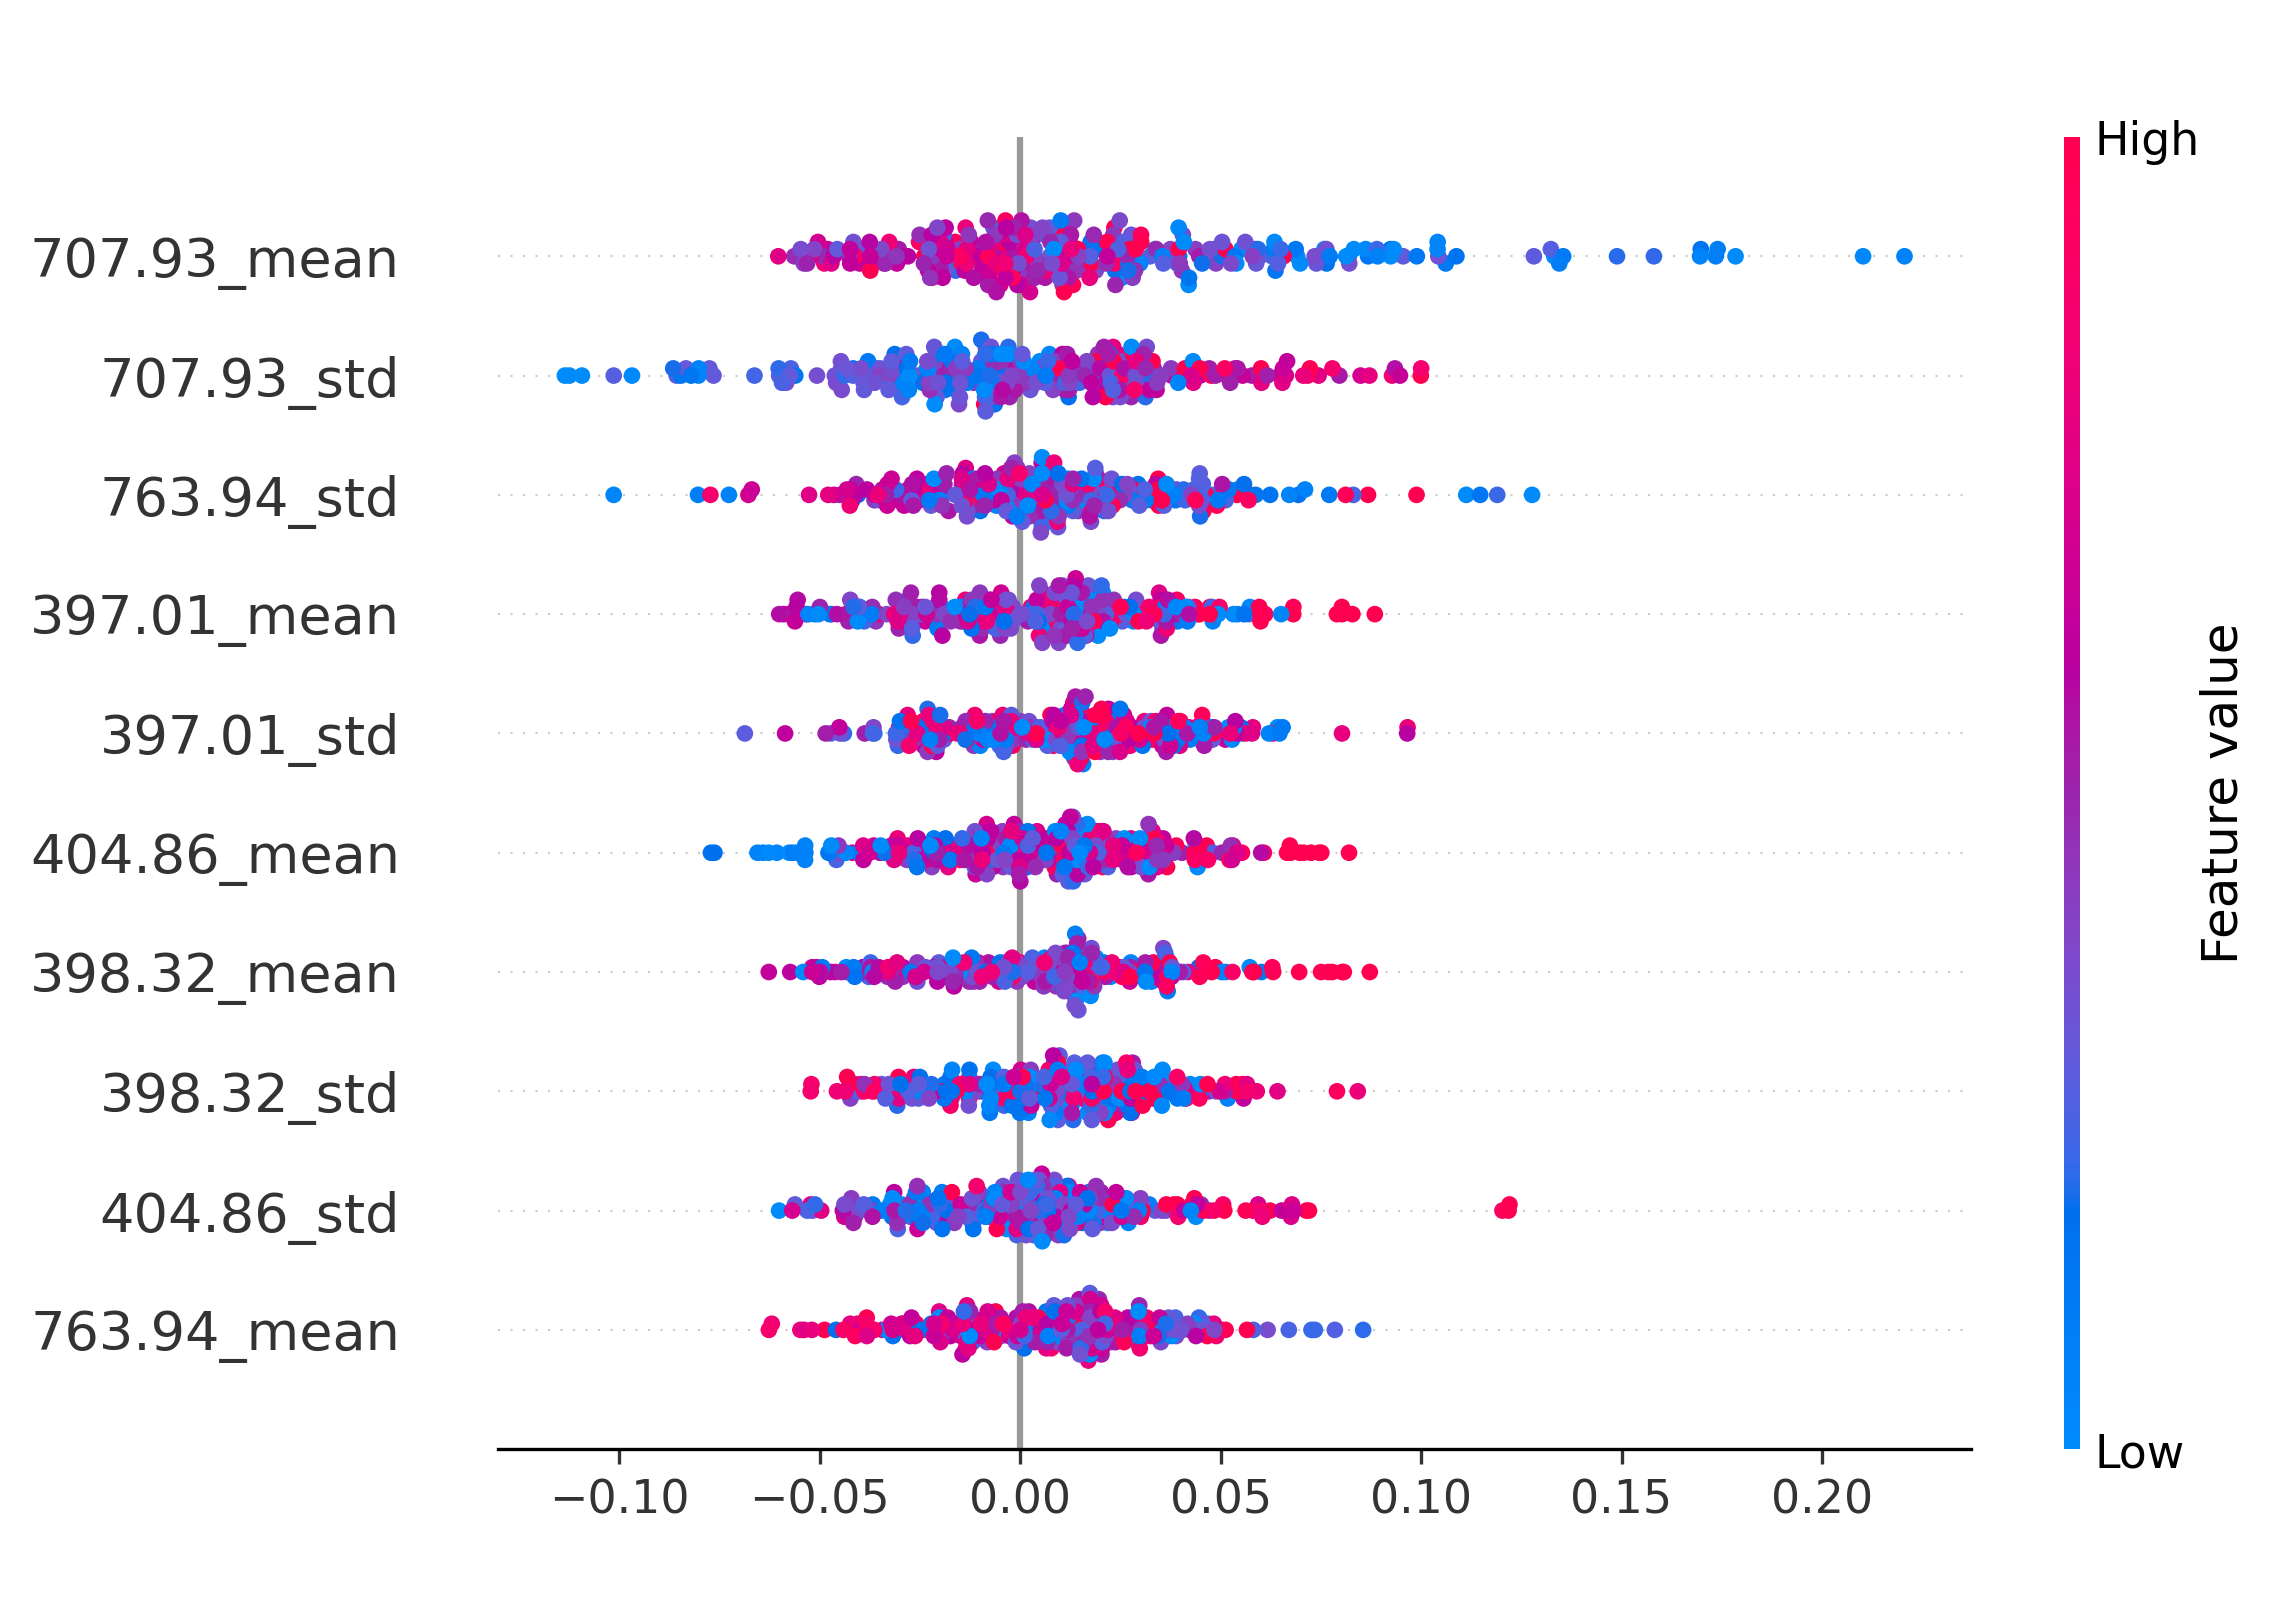
\includegraphics[width=0.5\textwidth]{images/shap_global_analysis_ga_5_bands.png}}
    \caption{Global explainability analysis (SHAP) for the optimal GA 5 band model. (a) Mean absolute feature importance ranking. (b) Beeswarm summary plot illustrating feature impact and directionality on the infected class. \label{fig:7}}
\end{figure}


\section{Conclusions}
This study presented a non-invasive methodology for the early detection of Aspergillus flavus in figs using hyperspectral imaging coupled with metaheuristic band selection. 
By constructing a statistical feature vector based on the spectral mean ($\mu$) and standard deviation ($\sigma$), the proposed approach successfully reduced the high dimensional hyperspectral data into a compact subset of informative characteristics. This subset of characteristics also captured successfully both spectral tendencies and textural heterogeneity induced by the infection. 
The experimental results demonstrated that the GA exhibited superior optimization capabilities compared to PSO. 

The GA identified an optimal, highly compact subset of only 5 bands \textit{(397.01, 398.32, 404.86, 707.93, and 763.94 nm)}, achieving a F1-Score of 0.836. 
Furthermore, the physical consistency of this optimal subset was validated. The algorithmically selected bands align exclusively with early visible pigmentation changes and structural markers induced by stress at the red edge \cite{mahlein_plant_2016}. Notably, the optimal model achieved maximum classification performance without relying on the water absorption region \textit{(950–1000 nm)}, proving that early pigment and textural stress markers are sufficiently discriminative for fungal detection \cite{nicolai_nondestructive_2007}. 

While the proposed framework demonstrates high efficacy in identifying severe \textit{Aspergillus flavus} infections ($10^7$ CFU/mL), this study is currently limited to scenarios with a high fungal load. Detecting the pathogen at lower inoculation concentrations (e.g., $10^3$ and $10^5$ CFU/mL) remains a more complex challenge, as these represent true early stage infections where structural degradation and pigment alterations are significantly less pronounced \cite{cruz-carrasco_detection_2024}. Therefore, future research will explicitly focus on evaluating this metaheuristic band selection approach on these lower concentration classes. Additionally, future work will explore multi-objective optimization algorithms to dynamically balance classification accuracy and subset dimensionality without predefined constraints, alongside advanced non-linear classifiers like XGBoost to further enhance the robustness of the spectral selection process.

\begin{credits}
\subsubsection{\ackname} This research is supported by Spanish Ministry of Science and Innovation under project PID2023-147409NB-C22 funded by MCIN-/AEI-/10.130-39/501100011033, Junta de Extremadura, project GR24142 and by “ERDF A way of making Europe”.

\subsubsection{\discintname}
The authors have no competing interests to declare that are
relevant to the content of this article.
\end{credits}

\bibliographystyle{splncs04}
\bibliography{refs}
\end{document}